%% CHAPTER HEADER /////////////////////////////////////////////////////////////////////////////////////
\chapter[The Severity of Damage Estimation]{The Severity of Damage Estimation}
\label{ch:severity}

%% CHAPTER INTRODUCTION ///////////////////////////////////////////////////////////////////////////////
A series of computer simulations were performed for different bond sizes for both the full and homogenised core model.
Two damage models were considered for both issues, i.e., the removed core cells  and no coupling between the core and the adhesive layer.
The electrical voltage signal captured at the sensor electrode was then analyzed to determine \ac{madif}.
Several \acp{di} were used to determine the effect of damage on the propagation waveform.
Of all the indices, the one with the lowest percentage error to experimental measurements will be selected to determine the \ac{madif}.
%% INCLUDE SECTIONS ///////////////////////////////////////////////////////////////////////////////////

%% SECTION HEADER /////////////////////////////////////////////////////////////////////////////////////
\section{Model-Assisted Damage Identification Function}
\label{sec:madif}

%% SECTION CONTENT ////////////////////////////////////////////////////////////////////////////////////
he severity of damage was estimated based on the function determined with the numerical simulation.
A simple flowchart given in Figure~\ref{fig:Flowchart} represents a process for the sample assessment.
When the structure model is developed, several computer simulations for various damage sizes must be conducted to determine the \ac{madif}.
%\begin{figure}[H]
%	%	\begin{center}
%	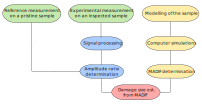
\includegraphics[width=1\linewidth]{Chapter_7/flowchart}
%	%	\end{center}
%	\caption{A flowchart representing the process for damage size estimation.}
%	\label{fig:Flowchart}
%\end{figure}
The \ac{madif} indicates the damage size according to measured damage index \(I\) normalized by the value obtained for the pristine sample \(I^{ref}\).
In the paper, two types of damage index \(I\) are considered: the energy \(I_{eng}\) and the maximum value of the half-width of the first package arrived in the sensor \(I_{amp}\), and these are defined as:
\begin{eqnarray}
	I_{eng}(\Phi_D)=\sum_{t=0}^{T} \left (\Psi_g(t,\Phi_D)\right )^2,\quad I_{eng}^{ref}=\sum_{t=0}^{T} \left (\Psi_g(t,0)\right )^2,\\
	I_{amp}(\Phi_D)=\mathrm{max}\left ( \Psi_g(t,\Phi_D)\right ),\quad I_{amp}^{ref}=\mathrm{max}\left ( \Psi_g(t,0)\right ),
	\label{eq:I_amp}
\end{eqnarray}
where \textit{T} is a period of the signal.
\(\Psi_g(t,\Phi_D)\) is for the damaged case scenario, whereas \(\Psi_g(t,0)\) is for the pristine sample and it is realized in the same way by windowing the full-length signals of the sensor \(\Psi(t)\) with a flattened Gaussian window \emph{g(t)} as follows:
\begin{eqnarray}
	\Psi_g(t)=\Psi(t)g(t)= \Psi(t)\mathrm{exp}\left(-\left(\frac{t-t_0}{0.6005612w_g}\right) ^{12}\right),
	\label{eq:psi_g}
\end{eqnarray}
where \(t_0\) is the center and \(w_g=0.5N_c/f_c\) is a half-width of the window.
Windowing the signals ensures obtaining the signals without any reflections from the boundaries.
The determination of \(\Psi_g\) is pictured in Figure~\ref{fig:window_madif}a.

\begin{figure}[H]
	%	\begin{center}
	\includegraphics[width=1\linewidth]{Chapter_7/window_madif_03}
	%	\end{center}
	\caption{(\textbf{a}) The %MDPI: The hyphen in the picture should be changed to minus sign, e.g., ``-0.5'' to ``$-$0.5'', please change. Please check all like this in all figures. 
		sensor signal \(\Psi(t)\) windowed by a flattened Gaussian window \(g(t)\) and (\textbf{b}) the damage size estimation from the \ac{madif}.}
	\label{fig:window_madif}
\end{figure}
In the time domain, an equivalent numerical signal to the signal registered by the \ac{pzt} acquisition instrument is calculated as an average value of the electrical potential of the electrode surface
\begin{eqnarray}
	\Psi^{n}(t) = \frac{\int_{\Gamma_e}\phi\mathrm{d}\Gamma}{\Gamma_e},
	\label{eq:psi}
\end{eqnarray}
where \(n=1\) and \(n=2\) correspond to the homogenized and presented model, respectively.

The \ac{madif} is achieved by approximating the inverse of the computed damage index that best matches the experimental one.
Finally, the damage size \(\Phi_D\) is obtained from the \ac{madif} curve for measuring the normalized value of \(I/I^{ref}\) as it is presented in Figure~\ref{fig:window_madif}b.
%% SECTION HEADER /////////////////////////////////////////////////////////////////////////////////////
\section{Determination of the \acs{madif}}
\label{sec:determination}

%% SECTION CONTENT ////////////////////////////////////////////////////////////////////////////////////
The \ac{madif} is determined based on the function best fitted to indices chosen in the previous subsection.
Since the numerically obtained indices take the shape of a non-linear function, several curves were assumed to find the best fit.
These functions are defined in the general form as follows:
\begin{eqnarray}
	y_1(x,a_i) & = & \frac{a_1x}{x+a_2}+a_3,
	\label{eq:function_1}\\
	y_2(x,a_i) & = & a_1\sqrt{x} + a_2x+a_3,
	\label{eq:function_2}\\
	y_3(x,a_i) & = & \frac{a_1x}{\sqrt{a_2 + a_3x^2}}+a_4,\label{eq:function_3} 
\end{eqnarray}
where \(a_i\) are the coefficients of the functions.
The coefficients are determined by built-in function of Matlab named \verb+fminsearch+, which searches for the minimum of a problem specified by \(\min\limits_a f(x,a)\), and the function to be optimised is assumed to be \(f(x,a)=\left\|DI_{num} - y(x,a_i)\right\|\), where \(\left\|\cdot\right\|\) means Euclidean norm.
A criterion for evaluating the fit of the curve to simulation results is a mean absolute error defined as the following:
\begin{eqnarray}
	\delta^{\mathrm{fit}} = \frac{1}{\mathrm{n^{DI}}}\sum_{i=1}^{\mathrm{n^{DI}}} \left|\frac{\mathrm{DI^i_{num}}-y(w_d^i)}{\mathrm{DI^i_{num}}}\right|\times100\%,
\end{eqnarray}
where \(\mathrm{n^{DI}}\) is the number of index points.
The examples of the results for \ac{rmsd} are presented in Tab.~\ref{tab:fit_RMSD_full_FCGM} based on the \ac{fcgm} and in Tab. \ref{tab:fit_RMSD_full_HCGM} for the \ac{hcgm}.
The empty cells in the tables mean that the function has been fitted with an error of more than 20\%.
The \ac{di} is no longer taken into account if the fit function has not been established.
A similar summary has been prepared for the remaining cases, but their presentation has been omitted for chapter clarity.
It turns out that the most fitted function is Eq.~(\ref{eq:function_1}) and Eq.~(\ref{eq:function_2}) for the most \acp{di}.
The best fitted functions were chosen for the \ac{madif} determination.

\begin{table}
	\small
	\tabcolsep=0.1cm
	\centering
	\caption{\label{tab:fit_RMSD_full_FCGM} The errors of the functions fitted to \acf{rmsd} based on full-length windowed signals and the \acf{fcgm}.}
	\begin{tabular}{ccccccccccccccc}
		\toprule
		\multirow{3}{*}{\rotatebox[origin=c]{90}{Frequency}} & \multicolumn{7}{c}{\ac{fcgm} - core} & \multicolumn{7}{c}{\ac{fcgm} - interface}\\
		& \multirow{2}{*}{\rotatebox[origin=c]{90}{DI\(_{num}\)}} & \multicolumn{2}{c}{Eq.~(\ref{eq:function_1})} & \multicolumn{2}{c}{Eq.~(\ref{eq:function_2})} & \multicolumn{2}{c}{Eq.~(\ref{eq:function_3})} &
		\multirow{2}{*}{\rotatebox[origin=c]{90}{DI\(_{num}\)}} & \multicolumn{2}{c}{Eq.~(\ref{eq:function_1})} & \multicolumn{2}{c}{Eq.~(\ref{eq:function_2})} & \multicolumn{2}{c}{Eq.~(\ref{eq:function_3})}\\
		& & \(y(w_d^i)\)& \(\delta^{\mathrm{fit}}\) & \(y(w_d^i)\) & \(\delta^{\mathrm{fit}}\) & \(y(w_d^i)\) & \(\delta^{\mathrm{fit}}\) & & \(y(w_d^i)\)& \(\delta^{\mathrm{fit}}\) & \(y(w_d^i)\) & \(\delta^{\mathrm{fit}}\) & \(y(w_d^i)\) & \(\delta^{\mathrm{fit}}\)\\
		\midrule
		\multirow{7}{*}{\rotatebox[origin=c]{90}{100 \unit{\kHz}}} & 1.00 & 1.00 & \multirow{7}{*}{\rotatebox[origin=c]{90}{\textcolor{green}{1.50}}} & 1.00 & \multirow{7}{*}{\rotatebox[origin=c]{90}{1.70}} & 1.00 & \multirow{7}{*}{\rotatebox[origin=c]{90}{1.92}} & 1.00 & 1.00 & \multirow{7}{*}{\rotatebox[origin=c]{90}{\textcolor{green}{1.11}}} & 1.00 & \multirow{7}{*}{\rotatebox[origin=c]{90}{1.45}} & 1.00 & \multirow{7}{*}{\rotatebox[origin=c]{90}{1.31}} \\
		& 0.83 & 0.85 & & 0.88 & & 0.84 & & 0.92 & 0.92 & & 0.90 & & 0.94 & \\ 
		& 0.82 & 0.80 & & 0.82 & & 0.79 & & 0.85 & 0.84 & & 0.83 & & 0.85 & \\ 
		& 0.80 & 0.78 & & 0.79 & & 0.78 & & 0.79 & 0.79 & & 0.79 & & 0.80 & \\ 
		& 0.76 & 0.78 & & 0.78 & & 0.78 & & 0.76 & 0.77 & & 0.76 & & 0.77 & \\ 
		& 0.77 & 0.77 & & 0.77 & & 0.78 & & 0.73 & 0.75 & & 0.74 & & 0.76 & \\ 
		& 0.75 & 0.77 & & 0.78 & & 0.78 & & 0.75 & 0.73 & & 0.72 & & 0.75 & \\
		\midrule
		\multirow{7}{*}{\rotatebox[origin=c]{90}{150 \unit{\kHz}}} & 1.00 & 1.00 & \multirow{7}{*}{\rotatebox[origin=c]{90}{3.10}} & 1.00 & \multirow{7}{*}{\rotatebox[origin=c]{90}{\textcolor{green}{1.28}}} & 1.00 & \multirow{7}{*}{\rotatebox[origin=c]{90}{6.83}} & 1.00 & 1.00 & \multirow{7}{*}{\rotatebox[origin=c]{90}{1.32}} & 1.00 & \multirow{7}{*}{\rotatebox[origin=c]{90}{\textcolor{green}{0.73}}} & 1.00 & \multirow{7}{*}{\rotatebox[origin=c]{90}{4.85}} \\
		& 0.89 & 0.95 & & 0.92 & & 0.97 & & 0.93 & 0.96 & & 0.95 & & 0.97 & \\ 
		& 0.85 & 0.87 & & 0.85 & & 0.91 & & 0.89 & 0.89 & & 0.88 & & 0.92 & \\ 
		& 0.80 & 0.81 & & 0.79 & & 0.85 & & 0.83 & 0.83 & & 0.82 & & 0.87 & \\ 
		& 0.74 & 0.76 & & 0.74 & & 0.80 & & 0.76 & 0.77 & & 0.77 & & 0.82 & \\ 
		& 0.68 & 0.71 & & 0.70 & & 0.75 & & 0.71 & 0.72 & & 0.72 & & 0.76 & \\ 
		& 0.64 & 0.67 & & 0.65 & & 0.70 & & 0.67 & 0.68 & & 0.67 & & 0.71 & \\ 
		\bottomrule
	\end{tabular}
\end{table}

\begin{table}
	\small
	\tabcolsep=0.1cm
	\centering
	\caption{\label{tab:fit_RMSD_full_HCGM} The errors of the functions fitted to \acf{rmsd} based on full-length windowed signals and the \acf{hcgm}.}
	\begin{tabular}{ccccccccccccccc}
		\toprule
		\multirow{3}{*}{\rotatebox[origin=c]{90}{Frequency}} & \multicolumn{7}{c}{\ac{hcgm} - core} & \multicolumn{7}{c}{\ac{hcgm} - interface}\\
		& \multirow{2}{*}{\rotatebox[origin=c]{90}{DI\(_{num}\)}} & \multicolumn{2}{c}{Eq.~(\ref{eq:function_1})} & \multicolumn{2}{c}{Eq.~(\ref{eq:function_2})} & \multicolumn{2}{c}{Eq.~(\ref{eq:function_3})} &
		\multirow{2}{*}{\rotatebox[origin=c]{90}{DI\(_{num}\)}} & \multicolumn{2}{c}{Eq.~(\ref{eq:function_1})} & \multicolumn{2}{c}{Eq.~(\ref{eq:function_2})} & \multicolumn{2}{c}{Eq.~(\ref{eq:function_3})}\\
		& & \(y(w_d^i)\)& \(\delta^{\mathrm{fit}}\) & \(y(w_d^i)\) & \(\delta^{\mathrm{fit}}\) & \(y(w_d^i)\) & \(\delta^{\mathrm{fit}}\) & & \(y(w_d^i)\)& \(\delta^{\mathrm{fit}}\) & \(y(w_d^i)\) & \(\delta^{\mathrm{fit}}\) & \(y(w_d^i)\) & \(\delta^{\mathrm{fit}}\)\\
		\midrule
		\multirow{7}{*}{\rotatebox[origin=c]{90}{100 \unit{\kHz}}} & 1.00 & 1.00 & \multirow{7}{*}{\rotatebox[origin=c]{90}{\textcolor{green}{5.37}}} & 1.00 & \multirow{7}{*}{\rotatebox[origin=c]{90}{9.85}} & \multirow{7}{*}{-} & \multirow{7}{*}{-} & 1.00 & 1.00 & \multirow{7}{*}{\rotatebox[origin=c]{90}{7.40}} & 1.00 & \multirow{7}{*}{\rotatebox[origin=c]{90}{\textcolor{green}{6.22}}} & 1.00 & \multirow{7}{*}{\rotatebox[origin=c]{90}{11.15}} \\
		& 0.55 & 0.57 & & 0.71 & & & & 0.67 & 0.75 & & 0.74 & & 0.80 & \\ 
		& 0.57 & 0.53 & & 0.58 & & & & 0.61 & 0.57 & & 0.59 & & 0.58 & \\ 
		& 0.57 & 0.52 & & 0.54 & & & & 0.53 & 0.50 & & 0.51 & & 0.51 & \\ 
		& 0.48 & 0.51 & & 0.52 & & & & 0.45 & 0.46 & & 0.46 & & 0.48 & \\ 
		& 0.50 & 0.51 & & 0.53 & & & & 0.35 & 0.44 & & 0.42 & & 0.47 & \\ 
		& 0.47 & 0.51 & & 0.55 & & & & 0.42 & 0.42 & & 0.40 & & 0.46 & \\ 
		\midrule
		\multirow{7}{*}{\rotatebox[origin=c]{90}{150 \unit{\kHz}}} & 1.00 & 1.00 & \multirow{7}{*}{\rotatebox[origin=c]{90}{0.51}} & 1.00 & \multirow{7}{*}{\rotatebox[origin=c]{90}{\textcolor{green}{0.33}}} & 1.00 & \multirow{7}{*}{\rotatebox[origin=c]{90}{2.41}} & 1.00 & 1.00 & \multirow{7}{*}{\rotatebox[origin=c]{90}{\textcolor{green}{0.79}}} & 1.00 & \multirow{7}{*}{\rotatebox[origin=c]{90}{\textcolor{green}{0.79}}} & \multirow{7}{*}{-} & \multirow{7}{*}{-} \\
		& 0.96 & 0.97 & & 0.97 & & 0.98 & & 0.95 & 0.95 & & 0.94 & & & \\ 
		& 0.93 & 0.93 & & 0.93 & & 0.95 & & 0.88 & 0.89 & & 0.89 & & & \\ 
		& 0.89 & 0.89 & & 0.89 & & 0.91 & & 0.84 & 0.85 & & 0.85 & & & \\ 
		& 0.85 & 0.85 & & 0.85 & & 0.88 & & 0.82 & 0.82 & & 0.82 & & & \\ 
		& 0.81 & 0.81 & & 0.81 & & 0.84 & & 0.80 & 0.79 & & 0.79 & & & \\ 
		& 0.77 & 0.78 & & 0.78 & & 0.80 & & 0.76 & 0.77 & & 0.76 & & & \\ 
		\bottomrule
	\end{tabular}
\end{table}

Then all chosen \acp{di} and their fitted functions are compared with experimental results.
The best results were obtained for the \ac{rmsd} and \ac{cc} based on the full-length signals at 100 \unit{kHz}. 
Those indices are presented in Fig.~\ref{fig:madif_rmsd_best} and Fig.~\ref{fig:madif_cc_best}, respectively.
\begin{figure}
	\begin{center}
		\includegraphics[width=0.95\textwidth]{Chapter_7/MADIF_RMSD_100_best_err}
	\end{center}
	\caption{ \textbf{(a)} Comparison of the \acf{madif} based on \acf{rmsd} and the experimental results, and \textbf{(b)} the percentage error between them.}
	\label{fig:madif_rmsd_best}
\end{figure}

\begin{figure}
	\begin{center}
		\includegraphics[width=0.95\textwidth]{Chapter_7/MADIF_CC_100_best_err}
	\end{center}
	\caption{\textbf{(a)} Comparison of the \acf{madif} based on \acf{cc} and the experimental results, and \textbf{(b)} the percentage error between them.}
	\label{fig:madif_cc_best}
\end{figure}
Both indices achieved the lowest error around 5\% for the \ac{fcgm}, with the interface elements removed as the damage model.
The indices are also in very good agreement for the \ac{fcgm} with removed cells as a damage model.
In the case of \ac{hcgm}, unsatisfactory results are obtained, as none of the indices correspond to the experimental ones with an error of less than 20\%.
What may be relevant here is that the wave transmits energy to the core throughout its propagation.
In contrast, in the case of \ac{fcgm}, the wave transmits energy incidentally, encountering cell walls.

According to the analysis, the \ac{rmsd} and \ac{cc} based on \ac{fcgm} and full-length signals at 100 \unit{kHz} were chosen as the \ac{madif}.
From Eq. \ref{eq:function_1}, they are defined as:
\begin{eqnarray}
	MADIF^{RMSD}(w_d) & = & {1.2695w_d}/(w_d+25.4048)+0.95,
	\label{eq:MADIF_RMSD}\\
	MADIF^{CC}(w_d) & = & 1.6091w_d/(w_d+6.6010)+0.7562,
	\label{eq:MADIF_CC}
\end{eqnarray}

The comparison of the \ac{madif} and the \ac{edif} based on \ac{rmsd} and \ac{cc} are presented in Fig.~\ref{fig:madif_20}.
The \ac{edif} was found using the fit function from Eq.~(\ref{eq:function_1}), the same as the \ac{madif}, for the \acp{di} based on experimental measurements.
The \ac{rmsd} is in excellent agreement with experiment, achieving an absolute error of less than 4 mm over the full range of damage.
For the \ac{cc}, the result is not as good as the previous one, but it also agrees with the experiment.
The absolute error is less than 9 mm.
Both indices can be used to estimate the damage size in the assumed scenario with a proposed approximation function.
\begin{figure}[!tbh]
	\begin{center}
		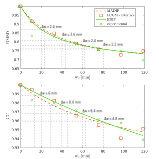
\includegraphics[width=1.0\textwidth]{Chapter_7/MADIF_20}
	\end{center}
	\caption{The \acf{madif} and the \acf{edif} based on the \acf{rmsd} 100 \unit{\kHz}.}
	\label{fig:madif_20}
\end{figure}
\clearpage
%%% SECTION HEADER /////////////////////////////////////////////////////////////////////////////////////
\section{Temperature Compensation}
\label{sec:compensation}

%% SECTION CONTENT ////////////////////////////////////////////////////////////////////////////////////

%% SECTION HEADER /////////////////////////////////////////////////////////////////////////////////////
\section{Conclusions}
\label{sec:conclusionsSever}

%% SECTION CONTENT ////////////////////////////////////////////////////////////////////////////////////
In the chapter, the \ac{madif} was determined by which the milestone of the dissertation was achieved.
For this purpose, four damage indicators were analysed for two different models of the panel core, two of which proved useless.
From among them, the one that best matched the measurements was selected to determine the function.
The numerical results are in good agreement with the experimental measurements.
It demonstrates the confirmation of the thesis that it is possible to determine the damage severity function in \ac{hsc} by employing numerical simulations.